\documentclass[a4paper,12pt,eval,firamath]{nsi}
\titre{Contrôle 03}
\classe{NSI2}
\begin{document}
\maketitle

\section*{Exercice 1 \small (bac 2021)}
\resetquestion
\textit{Cet exercice porte sur les arbres binaires de recherche, la programmation orientée
      objet et la récursivité.}\\

Dans cet exercice, la taille d'un arbre est le nombre de nœuds qu'il contient. Sa hauteur
est le nombre de nœuds du plus long chemin qui joint le nœud racine à l'une des
feuilles (nœuds sans sous-arbres). On convient que la hauteur d'un arbre ne contenant
qu'un nœud vaut 1 et la hauteur de l'arbre vide vaut 0.\\

On considère l'arbre binaire représenté ci-dessous:
\begin{center}
      
\includegraphics[width=7cm]{img/fig1.png}\\
      Figure 1
\end{center}
Donner la taille et la hauteur de cet arbre.\\

\carreauxseyes{16.8}{2.4}\\

\question Représenter ci-dessous le sous-arbre droit du n\oe ud de valeur 15.\\

\begin{tikzpicture}
      \draw (0,0) rectangle (\linewidth,5);
\end{tikzpicture}

\question Justifier que l'arbre de la figure 1 est un arbre binaire de recherche.\\

\carreauxseyes{16.8}{3.2}\\


On insère la valeur 17 dans l'arbre de la figure 1 de telle sorte que 17 soit une
nouvelle feuille de l'arbre et que le nouvel arbre obtenu soit encore un arbre
binaire de recherche.\\

\question Représenter ci-dessous ce nouvel arbre.\\

\begin{tikzpicture}
      \draw (0,0) rectangle (\linewidth,7);
\end{tikzpicture}
On considère la classe \mintinline{python}{Noeud} définie de la façon suivante en Python :


\begin{minted}{python}
        class Noeud:
            def __init__(self, g, v, d):
                self.gauche = g
                self.valeur = v
                self.droit = d
\end{minted}

\question Parmi les trois instructions suivantes, entourer celle qui construit et stocke dans la variable abr l'arbre représenté ci-dessous.
\begin{center}
      
\includegraphics[width=6cm]{img/fig1}
\end{center}


\begin{minted}{python}
abr = Noeud(Noeud(Noeud(None, 13, None), 15, None), 21, None)
abr = Noeud(None, 13, Noeud(Noeud(None, 15, None), 21, None))
abr = Noeud(Noeud(None, 13, None), 15, Noeud(None, 21, None)) 
\end{minted}

La fonction \mintinline{python}{ins} ci-dessous qui
prend en paramètres une valeur \mintinline{python}{v} et un arbre binaire de recherche \mintinline{python}{abr} et qui
renvoie l'arbre obtenu suite à l'insertion de la valeur \mintinline{python}{v} dans l'arbre \mintinline{python}{abr}.

Les lignes 8 et 9 permettent de ne pas insérer la valeur \mintinline{python}{v} si celle-ci est déjà présente dans \mintinline{python}{abr}.


\begin{minted}[linenos=true]{python}
        def ins(v, abr):
          if abr is None:
              return Noeud(None, v, None)
          if v > abr.valeur:
              return Noeud(abr.gauche, abr.valeur, ins(v, abr.droit))
          elif v < abr.valeur:
              return ............................................
          else:
          return abr      
      \end{minted}

\question Compléter le code de la fonction \mintinline{python}{ins}.\\



La fonction \mintinline{python}{nb_sup} ci dessous prend en paramètres une valeur \mintinline{python}{v} et un arbre binaire de recherche \mintinline{python}{abr} et renvoie le nombre de valeurs supérieures ou égales à la valeur \mintinline{python}{v} dans l'arbre \mintinline{python}{abr}.\\
Le code de cette fonction \mintinline{python}{nb_sup} est donné ci-dessous :

\begin{minted}{python}
def nb_sup(v, abr):
    if abr is None:
        return 0
    else:
        if abr.valeur >= v:
            return 1 + nb_sup(v, abr.gauche) + nb_sup(v, abr.droit)
        else:
            return nb_sup(v, abr.gauche) + nb_sup(v, abr.droit)
\end{minted}

On exécute l'instruction \mintinline{python}{nb_sup(16, abr)} dans laquelle \mintinline{python}{abr} est l'arbre initial de la figure 1.\\

\question Déterminer le nombre d'appels à la fonction \mintinline{python}{nb_sup} lors de cette exécution.\\

\carreauxseyes{16.8}{6.4}\\

L'arbre passé en paramètre étant un arbre binaire de recherche, on peut
améliorer la fonction \mintinline{python}{nb_sup} précédente afin de réduire ce nombre d'appels.\\

\question Écrire sur la copie le code modifié de cette fonction.\\

\carreauxseyes{16.8}{8}


\section*{Exercice 2 \small (bac 2023)}
\resetquestion
\textit{Cet exercice porte sur les arbres binaires, les files et la programmation orientée objet.
      Cet exercice comporte deux parties indépendantes.}\\

\subsection*{Partie 1}

Une entreprise stocke les identifiants de ses clients dans un arbre binaire de
recherche.\\
On rappelle qu'un arbre binaire est composé de nœuds, chacun des nœuds possédant
éventuellement un sous-arbre gauche et éventuellement un sous-arbre droit.\\
La taille d'un arbre est le nombre de nœuds qu'il contient. Sa hauteur est le nombre
de nœuds du plus long chemin qui joint le nœud racine à l'une des feuilles.
On convient que la hauteur d'un arbre ne contenant qu'un nœud vaut 1 et celle de
l'arbre vide vaut 0.\\
Dans cet arbre binaire de recherche, chaque nœud contient une valeur, ici une chaîne
de caractères, qui est, avec l'ordre lexicographique (celui du dictionnaire) :
\begin{itemize}
      \item strictement supérieure à toutes les valeurs des nœuds du sous-arbre gauche ;
      \item  strictement inférieure à toutes les valeurs des nœuds du sous-arbre droit.
\end{itemize}
Ainsi les valeurs de cet arbre sont toutes distinctes.
On considère l'arbre binaire de recherche suivant :
\begin{center}
      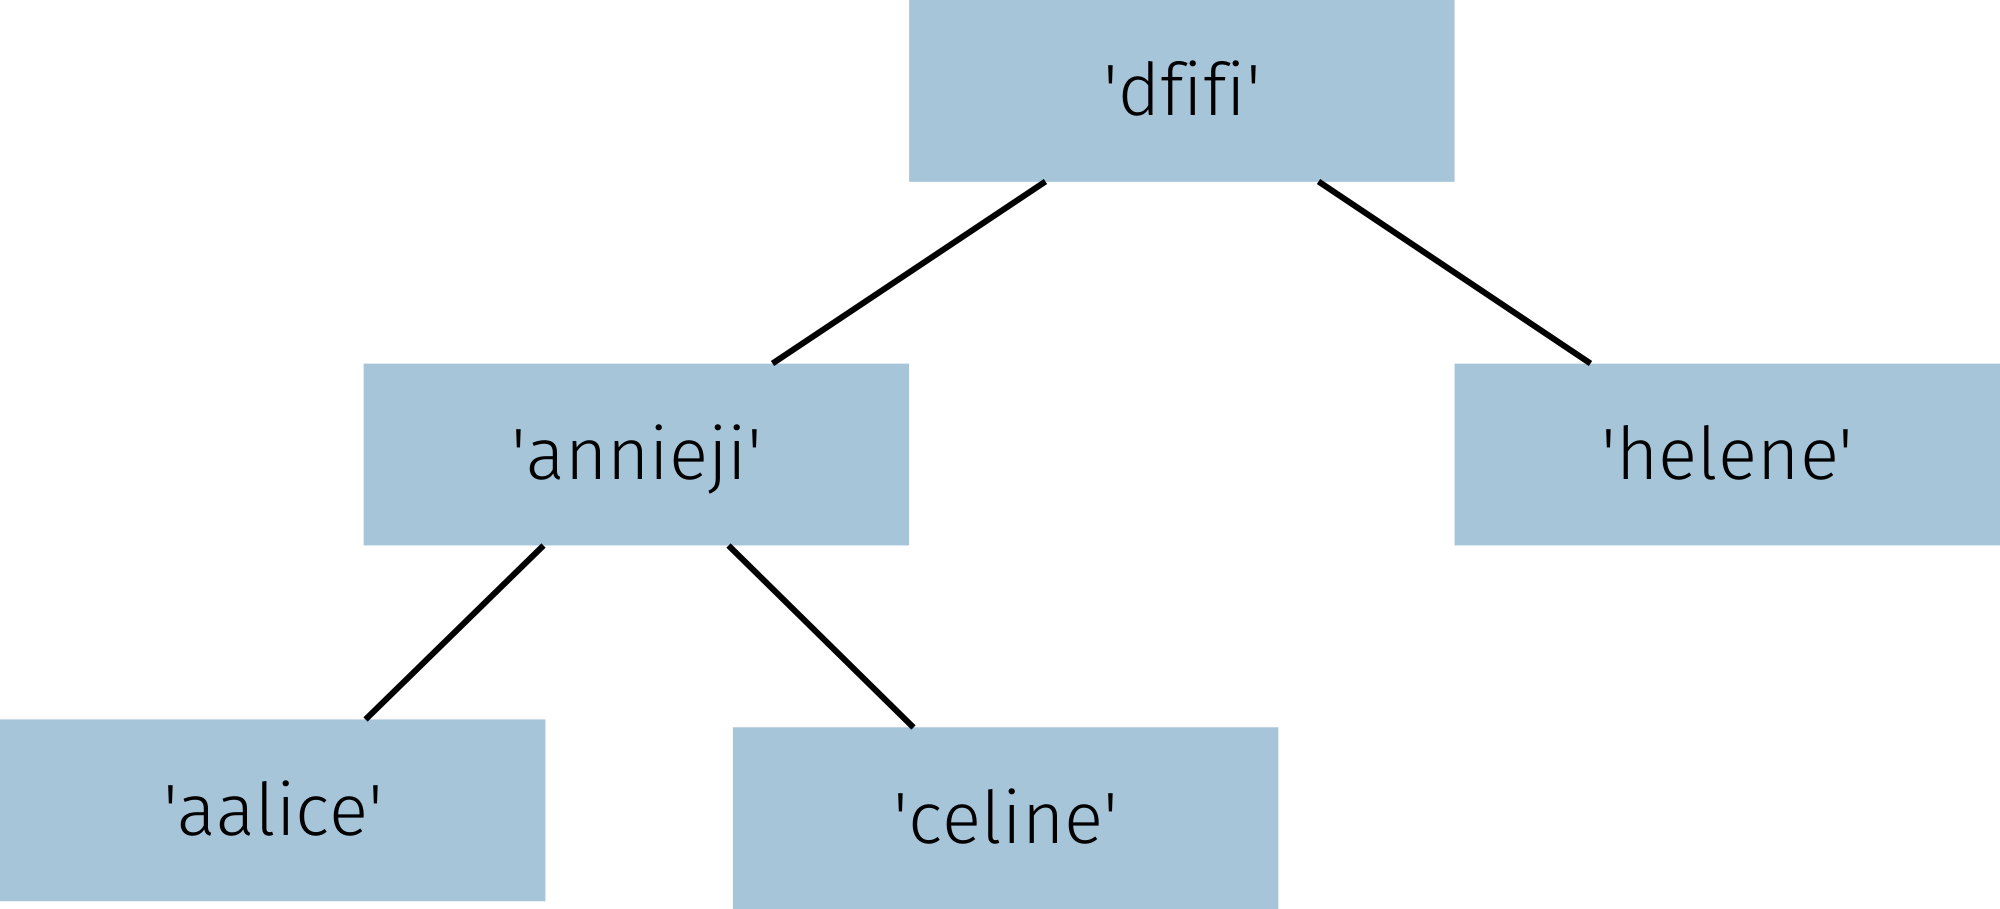
\includegraphics[width=7cm]{img/fig01.png}
\end{center}

\question Donner sa taille et sa hauteur.\\

\carreauxseyes{16.8}{1.6}\\

\question Recopier ci-dessous cet arbre après l'ajout des identifiants suivants : \mintinline{python}{'davidbg'}  et \mintinline{python}{'papicoeur'} dans cet ordre.\\

\begin{tikzpicture}
      \draw (0,0) rectangle (\linewidth,5);
\end{tikzpicture}

\question On décide de parcourir cet arbre pour obtenir la liste des identifiants dans l'ordre
lexicographique. Quel parcours doit-on utiliser ?\\

\carreauxseyes{16.8}{1.6}\\

Pour traiter informatiquement les arbres binaires, nous allons utiliser une classe
\mintinline{python}{ABR} .\\
Un arbre binaire de recherche, nommé \mintinline{python}{abr}  dispose des méthodes suivantes :
\begin{itemize}
      \item \mintinline{python}{abr.est_vide()} : renvoie \mintinline{python}{True}  si \mintinline{python}{abr} est vide et \mintinline{python}{False} sinon.
      \item \mintinline{python}{abr.racine()} : renvoie l'élément situé à la racine de \mintinline{python}{abr}  si \mintinline{python}{abr} n'est pas vide et \mintinline{python}{None} sinon.
      \item \mintinline{python}{abr.sg()} : renvoie le sous-arbre gauche de \mintinline{python}{abr}  s'il existe et \mintinline{python}{None} sinon.
      \item \mintinline{python}{abr.sd()}: renvoie le sous-arbre droit de \mintinline{python}{abr} s'il existe et None sinon.
\end{itemize}

On a commencé à écrire une méthode récursive \mintinline{python}{present}  de la classe \mintinline{python}{ABR}, où le paramètre \mintinline{python}{identifiant}  est une chaîne de caractères et qui renvoie \mintinline{python}{True}  si \mintinline{python}{identifiant} est dans l'arbre et \mintinline{python}{False} sinon.\\

\question Compléter ce code
\begin{pyc}
      \begin{minted}{python}
        def present(self, identifiant):
            if self.est_vide():
                return False
            elif self.racine() == identifiant:
                return ...
            elif self.racine() < identifiant:
                return self.sd(). ...
            else:
                return ...
    \end{minted}
\end{pyc}
\subsection*{Partie 2}

On considère une structure de données file que l'on représentera par des éléments en
ligne, l'élément à droite étant la tête de la file et l'élément à gauche étant la queue de
la file.
On appellera \mintinline{python}{f1} la file suivante :
\begin{center}
      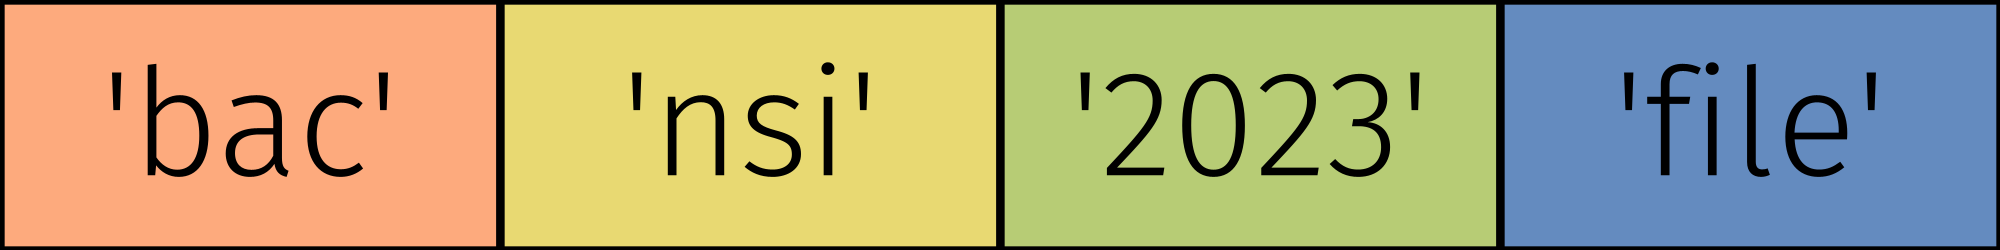
\includegraphics[width=6cm]{img/fig02.png}
\end{center}
On suppose que les quatre fonctions suivantes ont été programmées préalablement
en langage Python :
\begin{itemize}
      \item \mintinline{python}{creer_file()}  : renvoie une file vide ;
      \item \mintinline{python}{est_vide(f)}  : renvoie \mintinline{python}{True}  si la file \mintinline{python}{f}  est vide et \mintinline{python}{False}  sinon ;
      \item \mintinline{python}{enfiler(f, e)}  : ajoute l'élément \mintinline{python}{e}  à la queue de la file \mintinline{python}{f}  ;
      \item \mintinline{python}{defiler(f)}  : renvoie l'élément situé à la tête de la file \mintinline{python}{f}  et le retire de la file.
\end{itemize}

\question Donner le résultat renvoyé après l'appel de la fonction \mintinline{python}{est_vide(f1)}.\\

\carreauxseyes{16.8}{1.6}\\

\question Représenter la file \mintinline{python}{f1}  après l'exécution du code \mintinline{python}{defiler(f1)}.\\

\begin{tikzpicture}
      \draw (0,0) rectangle (\linewidth,2);
\end{tikzpicture}

\question Représenter la file \mintinline{python}{f2}  après l'exécution du code suivant :

\begin{pyc}
      \begin{minted}{python}
        f2 = creer_file()
        liste = ['castor', 'python', 'poule']
        for elt in liste:
            enfiler(f2, elt)
    \end{minted}
\end{pyc}

\begin{tikzpicture}
      \draw (0,0) rectangle (\linewidth,2);
\end{tikzpicture}

\question Compléter la fonction \mintinline{python}{longueur}  qui prend en
paramètre une file \mintinline{python}{f}  et qui renvoie le nombre d'éléments qu'elle contient.\\
Après un appel à la fonction, la file \mintinline{python}{f}  doit retrouver son état d'origine.\\

\begin{pyc}
      \begin{minted}{python}
        def longueur(f):
            resultat = 0
            g = creer_file()
            while ... :
                elt = defiler(f)
                resultat = ...
                enfiler(... , ...)
            while not(est_vide(g)):
                enfiler(f, defiler(g))
            return resultat
    \end{minted}
\end{pyc}

Un site impose à ses clients des critères sur leur mot de passe. Pour cela il utilise
la fonction \mintinline{python}{est_valide}  qui prend en paramètre une chaîne de caractères \mintinline{python}{mot}  et qui retourne \mintinline{python}{True}  si mot correspond aux critères et \mintinline{python}{False}  sinon.

\begin{pyc}
      \begin{minted}{python}
        def est_valide(mot):
            if len(mot) < 8:
                return False
            for c in mot:
                if c in ['!', '#', '@', ';', ':']:
                return True
            return False
    \end{minted}
\end{pyc}

\question Entourer le ou les mots validés par cette fonction.

\begin{itemize}
      \item \mintinline{python}{'best@'}
      \item 'paptap23'
      \item '2!@59fgds'
\end{itemize}

La figure suivante montre, sur deux exemples, l'évolution d'une file \mintinline{python}{f3}  après
l'exécution de l'instruction \mintinline{python}{ajouter_mot(f3, 'super')}  :
\begin{center}
      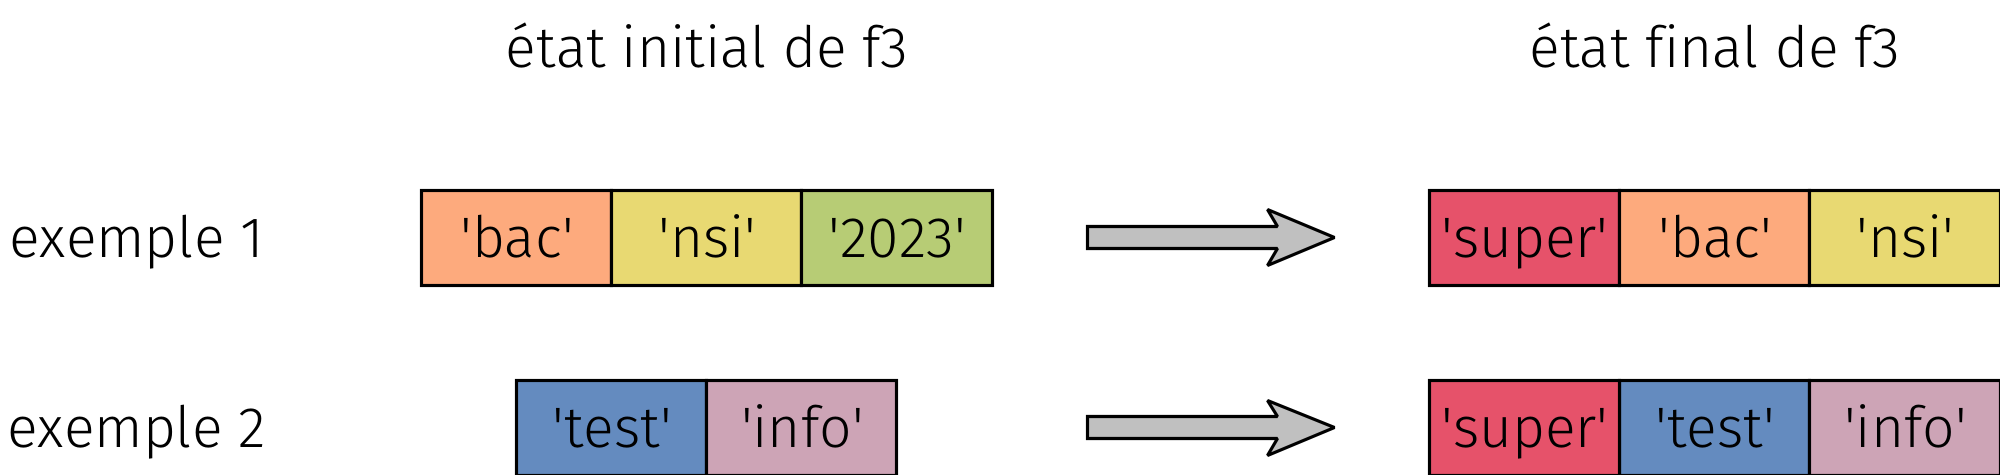
\includegraphics[width = 15cm]{img/fig03.png}
\end{center}

\question Écrire le code de cette fonction \mintinline{python}{ajouter_mot}  qui prend en paramètres une file \mintinline{python}{f}  (qui a au plus 3 éléments) et une chaîne de caractères valide \mintinline{python}{mdp} . Cette fonction met à jour la file de stockage \mintinline{python}{f}  des mots de passe en y ajoutant \mintinline{python}{mdp}  et en défilant, si nécessaire, pour avoir au maximum trois éléments dans cette file.\\
On pourra utiliser la fonction \mintinline{python}{longueur} définie précédemment.\\

\carreauxseyes{16.8}{8}\\

Pour intensifier sa sécurité, le site stocke les trois derniers mots de passe dans une
file et interdit au client lorsqu'il change son mot de passe d'utiliser l'un des mots de
passe stockés dans cette file.\\

\question Compléter la fonction \mintinline{python}{mot_file}  :
\begin{itemize}
      \item qui prend en paramètres une file \mintinline{python}{f}  et \mintinline{python}{mdp}  de type chaîne de caractères ;
      \item qui renvoie \mintinline{python}{True}  si le mot de passe est un élément de la file \mintinline{python}{f}  et \mintinline{python}{False} sinon.
\end{itemize}
Après un appel à cette fonction, la file \mintinline{python}{f}  doit retrouver son état d'origine.

\begin{pyc}
      \begin{minted}{python}
        def mot_file(f, mdp):
            g = creer_file()
            present = False
            while not(est_vide(f)):
                elt = defiler(f)
                enfiler(g, elt)
                if ...:
                    present = ...
            while not(est_vide(g)):
                enfiler(f, defiler(g))
            return present
    \end{minted}
\end{pyc}

\question Écrire une fonction \mintinline{python}{modification}  qui prend en paramètres une file \mintinline{python}{f}  et une chaîne de caractères \mintinline{python}{nv_mdp}.
Si le mot de passe \mintinline{python}{nv_mdp}  répond bien aux deux
exigences des questions \textbf{9.}  et \textbf{11.} , alors elle modifie la file des mots de passe stockés et
renvoie \mintinline{python}{True} . Dans le cas contraire, elle renvoie \mintinline{python}{False}.\\
On pourra utiliser les fonctions \mintinline{python}{mot_file} , \mintinline{python}{est_valide}  et \mintinline{python}{ajouter_mot}.

\carreauxseyes{16.8}{8}\\


\section*{Exercice 3 \small}

\resetquestion
On implémente une structure d'arbre binaire grâce à la classe \mintinline{python}{Node} du cours, dont voici un extrait :

\begin{pyc}
      \begin{minted}{python}
class Node:
     def __init__(self, v, left=None | int, right=None | int):
        self.value = v
        self.left = left  # vaut None ou bien un entier
        self.right = right  # vaut None ou bien un entier
\end{minted}
\end{pyc}

La notation \mintinline{python}{None | int}  signifie que le paramètre concerné peut être \mintinline{python}{None} ou une valeur de type \mintinline{python}{int}.\\


On aimerait savoir, étant donnée une instance de la classe \mintinline{python}{Node} nommée \mintinline{python}{root}, si l'arbre binaire de racine \mintinline{python}{root} est un ABR (arbre binaire de recherche). 

\question Rappeler quel parcours des n\oe uds d'un ABR permet d'obtenir les valeurs qu'ils contiennent dans l'ordre croissant et expliquer son fonctionnement.

\end{document}
